\documentclass[11pt]{article}

\usepackage[a4paper,margin=2.25cm]{geometry}
\usepackage{amsmath,amssymb,amsthm}
\usepackage{booktabs}
\usepackage{graphicx}
\usepackage[numbers,sort&compress]{natbib}
\usepackage{xcolor}
\usepackage{hyperref}

\graphicspath{{figures/}}
\hypersetup{
  colorlinks=true,
  linkcolor=blue,
  citecolor=blue,
  urlcolor=blue,
  pdftitle={Forecast-Calibrated Charger-Based Model Predictive Control for Unidirectional Workplace EV Charging},
  pdfauthor={Yizhan Gu}
}
\newtheorem{proposition}{Proposition}
\newcommand{\T}{\mathcal{T}}
\newcommand{\I}{\mathcal{I}}
\newcommand{\C}{\mathcal{C}}
\newcommand{\R}{\mathbb{R}}
\newcommand{\pos}[1]{\left[#1\right]_{+}}
\DeclareMathOperator*{\argmin}{arg\,min}

\title{\textbf{Forecast-Calibrated Charger-Based Model Predictive Control for
Unidirectional Workplace EV Charging}\\
\large Exact aggregation, continuous demand-charge accounting, and a
three-month out-of-sample pilot}
\author{Yizhan Gu\\
University of California San Diego, La Jolla, CA, USA}
\date{Draft generated July 26, 2026\\
\small Target journal: \emph{Sustainable Energy, Grids and Networks}}

\begin{document}
\maketitle

\begin{abstract}
This paper studies whether forecast uncertainty can create measurable economic
value in charger-based model predictive control (MPC) for unidirectional
workplace electric-vehicle charging.  The setting intentionally excludes
vehicle-to-grid export, battery storage, photovoltaics, and demand response;
therefore, economic value means avoided charging cost rather than market
revenue.  We first derive a sparse charger-level linear program whose
cumulative-energy envelopes are an exact projection of the session-level
problem when sessions do not overlap on a physical port.  The controller carries
executed noncoincident and on-peak demand states continuously through each
billing month, preventing the repeated daily demand-charge approximation that
can severely distort results.  A causal four-week same-weekday median forecast
is then corrected with one-sided split-conformal residuals for late arrival,
early departure, and underpredicted energy.  We evaluate six fixed UC San Diego
ports over 92 unseen days in July--September 2023.  All 552 day--method runs
serve the required energy without fallback.  The conformal controller costs
\$4,177.90, a 28.23\% reduction from immediate charging and a 1.47\% reduction
from point-forecast MPC; its regret to perfect information is 4.43\%.  Empirical
one-sided coverages are 91.5\%, 91.5\%, and 90.2\% against a 90\% target.
However, the conformal method improves only two of three billing months, so the
result is a reproducible pilot rather than evidence of statistical
generalization.  Synthetic tests preserve the EV-level objective to
\(1.14\times10^{-12}\) and give a median \(2.07\times\) speedup at eight
sessions per charger.
\end{abstract}

\noindent\textbf{Keywords:} electric-vehicle charging; charger aggregation;
model predictive control; conformal prediction; demand charges; forecast value

\section{Introduction}

Workplace EV charging is naturally a receding-horizon control problem: sessions
arrive throughout the day, their flexibility differs, and monthly demand
charges couple otherwise independent days.  Session-level optimization is
physically transparent but expands with the number of vehicles.  Charger-level
optimization is smaller, but a daily-energy-only aggregation can move energy
across a vehicle's arrival or deadline and consequently report false savings.
The first question in this work is therefore structural: under which operating
conditions is a charger representation both smaller and exactly feasible?

The second question concerns uncertainty.  Classical charging formulations
optimize known requests \citep{sortomme2011optimal,gan2013optimal}, whereas
closed-loop station control must act before later sessions are observed.
Stochastic EV-station models explicitly consider uncertain arrival, departure,
and energy \citep{puech2024controlling}.  Recent charging-hub MPC combines
machine-learning forecasts with conformal uncertainty sets and reports a
roughly 1\% improvement over deterministic point forecasts in a richer
PV--battery setting \citep{fernandez2025conformal}.  Here we isolate the
charger-control effect: there is no storage, PV, export, V2G, or demand-response
signal.

Our contributions are:
\begin{enumerate}
  \item an exact sparse charger projection for nonoverlapping physical-port
  sessions, together with an explicit disaggregation argument;
  \item a rolling MPC implementation that carries executed billing-peak states
  across days and evaluates only incremental monthly demand cost;
  \item a leakage-controlled comparison of no forecast, persistence,
  historical-median, one-sided conformal, and perfect-information forecasts;
  and
  \item numerical invariance, feasibility, coverage, and scalability audits
  that make the boundary of the current evidence explicit.
\end{enumerate}

\section{Physical and tariff model}
\subsection{Sets, data, and assumptions}

One day is divided into \(\T=\{1,\ldots,T\}\) intervals of length
\(\Delta t=0.25\) h; \(T=96\).  Let \(\C\) be the physical chargers and
\(\I_c\) the sessions assigned to charger \(c\).  Session \(i\) has arrival
\(a_i\), inclusive departure \(d_i\), requested grid energy \(E_i\), and maximum
power \(\bar p_i\).  Its availability set is
\[
  \T_i=\{t\in\T:a_i\le t\le d_i\}.
\]
Charging is unidirectional:
\[
  p_{i,t}\ge0.
\]
There is no export, stationary battery, PV, feeder-network constraint, or
demand-response payment.  Charging efficiency is already absorbed into the
metered energy request.  Once a session arrives, \(d_i,E_i,\bar p_i\) are
assumed observable.  Most importantly, sessions on each selected physical port
do not overlap:
\begin{equation}
  i,j\in\I_c,\ a_i<a_j \quad\Longrightarrow\quad d_i<a_j .
  \label{eq:nonoverlap}
\end{equation}
Equation~\eqref{eq:nonoverlap} is checked in data and before every optimization.

\subsection{Session-level reference problem}

The exact EV-level feasible set is
\begin{subequations}\label{eq:evfeasible}
\begin{align}
  0\le p_{i,t}&\le \bar p_i\mathbf{1}_{\{t\in\T_i\}},
    &&i\in\I,\ t\in\T, \label{eq:evpower}\\
  \Delta t\sum_{t\in\T_i}p_{i,t}&=E_i,
    &&i\in\I. \label{eq:evenergy}
\end{align}
\end{subequations}
The total site charging power is
\begin{equation}
  P_t=\sum_{i\in\I}p_{i,t}.                         \label{eq:siteload}
\end{equation}
This reference formulation is a linear program (LP) and is used only for
invariance and scalability comparisons, not for the rolling paper experiment.

\subsection{Exact charger-level cumulative envelopes}

Define cumulative delivered energy through interval \(t\) for session \(i\).
The greatest energy that could have been delivered is
\begin{equation}
  U_{i,t}=\min\!\left\{
    E_i,\ \bar p_i\Delta t\,
    \pos{\min(t,d_i)-a_i+1}
  \right\},                                        \label{eq:upper}
\end{equation}
and the least energy that must already have been delivered, leaving enough
future capacity, is
\begin{equation}
  L_{i,t}=\max\!\left\{
    0,\ E_i-\bar p_i\Delta t\,
    \pos{d_i-\max(t+1,a_i)+1}
  \right\}.                                        \label{eq:lower}
\end{equation}
Aggregate envelopes are \(U_{c,t}=\sum_{i\in\I_c}U_{i,t}\) and
\(L_{c,t}=\sum_{i\in\I_c}L_{i,t}\).  With charger power \(p_{c,t}\), introduce
the sparse cumulative state
\begin{subequations}\label{eq:charger}
\begin{align}
 e_{c,0}&=0,\\
 e_{c,t}&=e_{c,t-1}+\Delta t\,p_{c,t},
      &&c\in\C,\ t\in\T, \label{eq:state}\\
 L_{c,t}&\le e_{c,t}\le U_{c,t},
      &&c\in\C,\ t\in\T, \label{eq:envelope}\\
 0\le p_{c,t}&\le
 \sum_{i\in\I_c}\bar p_i\mathbf{1}_{\{t\in\T_i\}}.
      \label{eq:chargerpower}
\end{align}
\end{subequations}
Under~\eqref{eq:nonoverlap}, at most one term in the right side of
\eqref{eq:chargerpower} is nonzero.

\begin{proposition}[Exact charger projection]
If sessions on every physical port satisfy~\eqref{eq:nonoverlap}, the set of
aggregate trajectories satisfying~\eqref{eq:charger} is exactly the projection
of the session-level feasible set~\eqref{eq:evfeasible} under
\(p_{c,t}=\sum_{i\in\I_c}p_{i,t}\).
\end{proposition}

\begin{proof}
For any feasible session dispatch, summing its cumulative energy establishes
\eqref{eq:state}--\eqref{eq:envelope}; availability establishes
\eqref{eq:chargerpower}.  Conversely, nonoverlap means every occupied
charger--time pair has one unique active session.  Assign \(p_{c,t}\) to that
session and zero to all others.  The upper envelope prevents premature energy,
the lower envelope forces each completed session to have received \(E_i\), and
the pointwise bound enforces \(\bar p_i\).  At \(t=d_i\), both session envelopes
equal \(E_i\); because later sessions have not arrived, their cumulative
contribution is zero.  Hence each session energy equality holds and the
assignment is a feasible disaggregation.
\end{proof}

The recurrence~\eqref{eq:state} has \(O(|\C|T)\) nonzeros.  A dense prefix-sum
encoding has \(O(|\C|T^2)\) nonzeros even though it represents the same state.

\subsection{Continuous monthly tariff state}

Let \(\lambda_t\) be the time-of-use energy price and
\(\T^{\mathrm{on}}=\{65,\ldots,84\}\) the 16:00--21:00 on-peak intervals.
The implemented summer tariff uses \(\lambda_t=\$0.12628/\mathrm{kWh}\) on peak
and \(\$0.10679/\mathrm{kWh}\) otherwise, noncoincident demand rate
\(\kappa^N=\$24.48/\mathrm{kW}\), and on-peak demand rate
\(\kappa^P=\$28.92/\mathrm{kW}\).  Additional tariff coefficients are a
fraction \(\rho=0.0578\) and volumetric charge
\(\eta=\$0.00668/\mathrm{kWh}\).

For billing month \(m\), let \(z^N_{m,d-1}\) and \(z^P_{m,d-1}\) be the
\emph{executed} peaks before day \(d\).  Their recursion is
\begin{subequations}\label{eq:peakstate}
\begin{align}
 z^N_{m,d}&=\max\!\left\{z^N_{m,d-1},\max_{t\in\T}P_{d,t}\right\},\\
 z^P_{m,d}&=\max\!\left\{z^P_{m,d-1},
                  \max_{t\in\T^{\mathrm{on}}}P_{d,t}\right\}.
\end{align}
\end{subequations}
The day-\(d\) incremental bill contribution optimized and evaluated is
\begin{align}
 J_{m,d}={}&(1+\rho)\Delta t
     \sum_{t\in\T}\lambda_tP_{d,t}\nonumber\\
 &+(1+\rho)\kappa^N(z^N_{m,d}-z^N_{m,d-1})\nonumber\\
 &+(1+\rho)\kappa^P(z^P_{m,d}-z^P_{m,d-1})\nonumber\\
 &+\eta\Delta t\sum_{t\in\T}P_{d,t}.                \label{eq:cost}
\end{align}
Thus demand increments telescope:
\[
 \sum_{d\in m}\kappa^N(z^N_{m,d}-z^N_{m,d-1})
 =\kappa^N z^N_{m,D_m},
\]
and similarly on peak.  Treating each day as a fresh bill would instead charge
the demand maximum repeatedly and is not used in reported results.

\section{Forecast-calibrated rolling MPC}
\subsection{Causal point forecast}

For target day \(d\), the historical-median model uses only the same weekday in
the preceding \(K=4\) weeks.  For each charger \(c\), it predicts the number of
sessions by the rounded median of the four counts.  Sessions are ordered by
arrival on each historical day.  For ordinal \(j\), the point forecast is
\begin{equation}
 (\widehat a_{cjd},\widehat d_{cjd},\widehat E_{cjd},
 \widehat{\bar p}_{cjd})
 =\operatorname{median}_{\ell=1,\ldots,K}
 (a_{cj,d-7\ell},d_{cj,d-7\ell},E_{cj,d-7\ell},
 \bar p_{cj,d-7\ell}),                              \label{eq:median}
\end{equation}
using the available ordinal samples.  Windows are clipped to the day and
sequentially reconciled to retain port nonoverlap.

\subsection{One-sided split-conformal correction}

We calibrate failure-relevant residuals on ordinal-matched sessions:
\begin{equation}
 r^a_k=a_k-\widehat a_k,\qquad
 r^d_k=\widehat d_k-d_k,\qquad
 r^E_k=E_k-\widehat E_k .                            \label{eq:residuals}
\end{equation}
Positive values respectively mean later arrival, earlier departure, or larger
energy than forecast.  For a residual sample \(r_1,\ldots,r_n\), the
finite-sample one-sided split-conformal quantile is
\begin{equation}
 q_{1-\alpha}(r)=r_{(\,k\,)},\qquad
 k=\min\!\left\{n,\left\lceil(n+1)(1-\alpha)\right\rceil\right\},
                                                           \label{eq:quantile}
\end{equation}
where \(r_{(k)}\) is the \(k\)-th order statistic
\citep{shafer2008tutorial,romano2019conformalized}.  The robust session passed
to the deterministic MPC is
\begin{subequations}\label{eq:robust}
\begin{align}
 \widetilde a_i&=\min\{T,\widehat a_i+\max(0,q^a)\},\\
 \widetilde d_i&=\max\{\widetilde a_i,
                       \widehat d_i-\max(0,q^d)\},\\
 \widetilde E_i&=\min\{\widehat E_i+\max(0,q^E),
 \bar p_i\Delta t(\widetilde d_i-\widetilde a_i+1)\}.
\end{align}
\end{subequations}
This is a conservative forecast transformation, not a joint chance-constrained
program.  Marginal split-conformal coverage is expected under exchangeability;
the chronological experiment reports empirical coverage rather than asserting
that workplace sessions are exchangeable.  Count underprediction is measured
but no fictitious session is synthesized because its physical window and
energy would be unknown.

\subsection{Receding-horizon information pattern}

At interval \(t\), the work set contains (i) actual connected sessions rebased
to their remaining energy and (ii) forecasts whose predicted arrival is later
than \(t\).  Arrived truth supersedes any overlapping forecast on the same
charger.  The controller solves the charger LP with the current monthly peak
states, executes only the first action, updates delivered energy and
\eqref{eq:peakstate}, and repeats.  Planned power is never delivered unless an
actual EV is connected.  There is no post-hoc replacement of missed energy.
This follows the standard receding-horizon structure \citep{rawlings2017mpc}.

LPs can have many economically identical solutions.  For reproducible
EV/charger comparisons, every solve is lexicographic.  First,
\[
 J^\star=\min_{x\in\mathcal X}J(x).
\]
Then the controller chooses
\begin{equation}
 x^\star_{\mathrm{lex}}\in\argmin_{x\in\mathcal X}
 \sum_{c,t}\frac{t}{T}p_{c,t}
 \quad\text{s.t.}\quad
 J(x)\le J^\star+\epsilon_{\mathrm{lex}},             \label{eq:lex}
\end{equation}
where
\(\epsilon_{\mathrm{lex}}=\max(10^{-6},10^{-7}|J^\star|)\) USD.  The reported
objective is always the primary tariff cost.

\section{Experimental protocol}
\subsection{Data and leakage control}

The local UCSD charging table contains 340,060 sessions from July 20, 2016 to
September 16, 2024, covering 291 ports.  The paper pilot uses six fixed ports
and 808 sessions during July 1--September 30, 2023.  Ports are ranked by
activity and energy using May--June only; a data-quality screen additionally
requires nonoverlap throughout the loaded evaluation window.  This screen uses
test-period timestamps only to verify the structural assumption and does not
use test costs, energy magnitudes for ranking, or controller outcomes.

Hyperparameter selection is chronological.  Candidate
\(\alpha\in\{0.1,0.2,0.3,0.4\}\) values use April--May residual calibration and
June closed-loop validation.  After selecting \(\alpha=0.1\), the corrections
are refit on the immediately preceding May--June window, with the Q3 test
untouched.  The final 680 matched residuals give
\[
 q^a=17\text{ slots},\qquad q^d=18\text{ slots},\qquad
 q^E=13.6035\text{ kWh}.
\]
The 90th percentile count-underprediction residual is one session, but is
reported rather than converted to a synthetic request.

\subsection{Methods and metrics}

Six controllers share the same tariff, physical model, state update, and
solver:
\begin{itemize}
 \item \textbf{V0G}: immediate maximum-rate charging;
 \item \textbf{Perfect}: future actual sessions supplied as an unattainable
 information upper benchmark;
 \item \textbf{No forecast}: MPC knows a request only after it arrives;
 \item \textbf{Persistence}: sessions from the same weekday one week earlier;
 \item \textbf{Historical median}: the causal point forecast in
 \eqref{eq:median}; and
 \item \textbf{Conformal}: \eqref{eq:robust} applied to the historical median.
\end{itemize}
Cost savings and perfect-information regret are
\begin{equation}
 S_m=100\frac{J^{\mathrm{V0G}}_m-J_m}{J^{\mathrm{V0G}}_m},
 \qquad
 R_m=100\frac{J_m-J^{\mathrm{Perfect}}_m}
 {J^{\mathrm{Perfect}}_m}.                            \label{eq:metrics}
\end{equation}
Forecast errors are computed on ordinal-matched sessions; count mean absolute
error (MAE) is averaged per charger-day.  A run is accepted only if unserved
energy is below \(10^{-5}\) kWh, the solver reports optimality at every call,
fallback count is zero, and peak states are monotone within each month.

\section{Results}
\subsection{Control value and forecast calibration}

\begin{table}[t]
\centering
\caption{Out-of-sample control results, July--September 2023.  ``Cost'' is the
sum of continuous monthly tariff contributions, not a sum of isolated daily
demand bills.}
\label{tab:control}
\begin{tabular}{lrrr}
\toprule
Method & Q3 cost (USD) & Saving vs. V0G & Regret vs. perfect \\
\midrule
V0G & 5821.16 & 0.00\% & 45.50\% \\
Perfect & 4000.79 & 31.27\% & 0.00\% \\
No forecast & 4243.88 & 27.10\% & 6.08\% \\
Persistence & 4317.58 & 25.83\% & 7.92\% \\
Hist. median & 4240.03 & 27.16\% & 5.98\% \\
Conformal & 4177.90 & 28.23\% & 4.43\% \\
\bottomrule
\end{tabular}

\end{table}

Table~\ref{tab:control} shows that all MPC variants improve on V0G.  The
conformal controller reduces cost by 28.23\% relative to V0G, closes most of
the gap to perfect information, and costs 1.47\% less than historical-median
MPC:
\[
 100\frac{4240.03-4177.90}{4240.03}=1.465\%.
\]
Its monthly cost improvement over historical median is \$50.32 in July and
\$49.87 in August, but it is \$38.06 worse in September.  Three monthly pairs
are insufficient for a meaningful significance claim.

\begin{figure}[t]
\centering
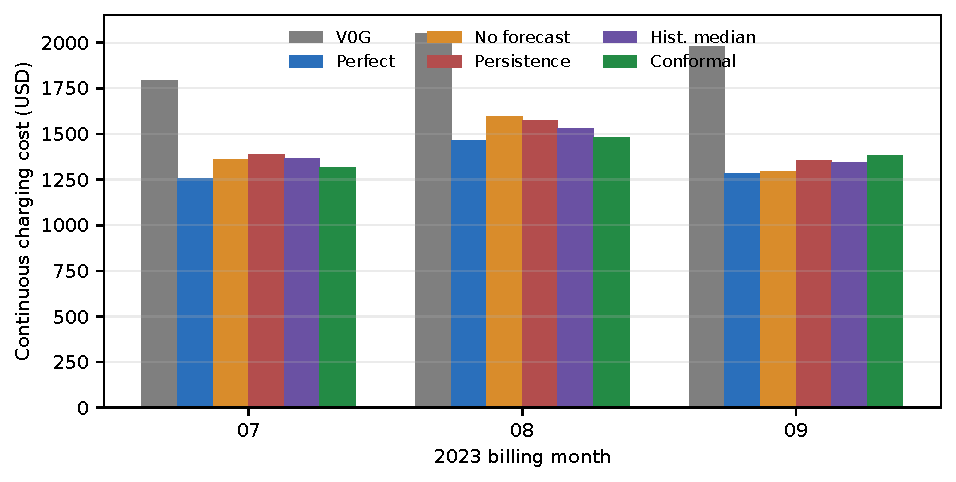
\includegraphics[width=\linewidth]{monthly_control_cost.pdf}
\caption{Continuous monthly charging cost.  Each method's executed peak state
is reset only at the billing-month boundary.}
\label{fig:monthly}
\end{figure}

\begin{table}[t]
\centering
\caption{Q3 session forecast diagnostics.  Arrival and departure MAE are in
15-minute slots.  Robust inputs are intentionally not point-forecast-optimal.}
\label{tab:forecast}
\begin{tabular}{lrrrr}
\toprule
Method & Count MAE & Arrival MAE & Departure MAE & Energy MAE \\
 & (sessions) & (slots) & (slots) & (kWh) \\
\midrule
Persistence & 0.962 & 10.783 & 11.744 & 8.031 \\
Hist. median & 0.868 & 9.366 & 10.687 & 6.811 \\
Conformal & 0.868 & 18.300 & 12.203 & 9.905 \\
\bottomrule
\end{tabular}

\end{table}

Historical median improves every point metric over persistence
(Table~\ref{tab:forecast}).  The robust transformation increases point MAE,
which is expected because its purpose is one-sided risk protection rather than
conditional-median accuracy.  Against the historical-median point forecast,
empirical one-sided coverage is 91.48\% for late arrival, 91.48\% for early
departure, and 90.16\% for energy underprediction, close to or above the 90\%
target.

\begin{figure}[t]
\centering
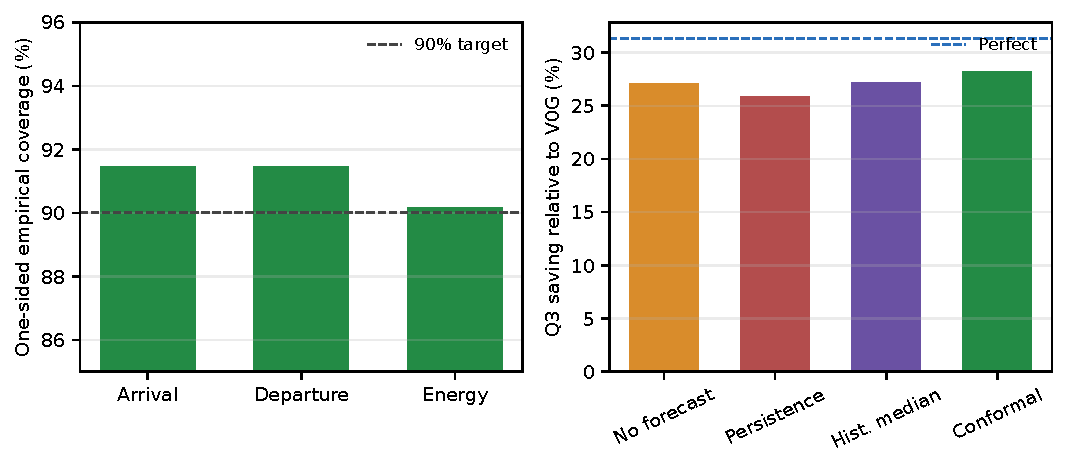
\includegraphics[width=\linewidth]{coverage_and_control_value.pdf}
\caption{Left: empirical one-sided Q3 coverage of conformal corrections.
Right: Q3 saving relative to V0G; the dashed line is perfect information.}
\label{fig:coverage}
\end{figure}

\begin{table}[t]
\centering
\caption{Chronological June validation used to select \(\alpha\).  June is
never part of the Q3 test.}
\label{tab:alpha}
\begin{tabular}{lrr}
\toprule
$\alpha$ & Nominal coverage & June validation cost (USD) \\
\midrule
0.1 & 90\% & 1603.32 \\
0.2 & 80\% & 1628.86 \\
0.3 & 70\% & 1636.76 \\
0.4 & 60\% & 1737.04 \\
\bottomrule
\end{tabular}

\end{table}

The validation ranking in Table~\ref{tab:alpha} selects the most conservative
candidate.  This does not imply that lower \(\alpha\) must always be cheaper:
shrinking windows and increasing energy can also create excessive early
charging and higher peaks.

\subsection{Exactness and computational scaling}

On 28 real-day comparisons, EV- and charger-level LPs have maximum absolute
objective difference \(1.14\times10^{-12}\) USD and maximum aggregate-load
difference \(7.64\times10^{-11}\) kW after the common lexicographic tie-break.
Every charger trajectory disaggregates to sessions with exact requested energy.

\begin{table}[t]
\centering
\caption{EV/charger invariance and synthetic scaling diagnostics.}
\label{tab:scaling}
\begin{tabular}{lr}
\toprule
Diagnostic & Value \\
\midrule
Maximum absolute objective gap & 1.14e-12 \\
Maximum aggregate-load gap (kW) & 7.64e-11 \\
Median synthetic speedup at 8 sessions/charger & 2.07$\times$ \\
\bottomrule
\end{tabular}

\end{table}

\begin{figure}[t]
\centering
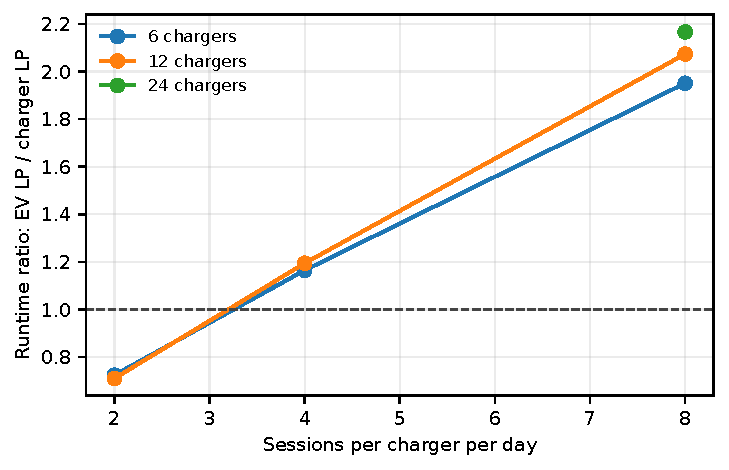
\includegraphics[width=0.78\linewidth]{synthetic_scalability.pdf}
\caption{Median runtime ratio of the EV LP to the exact sparse charger LP.
Aggregation becomes beneficial as sessions per charger increase; at low
density, charger cumulative states can outweigh variable reduction.}
\label{fig:scaling}
\end{figure}

The charger formulation is not uniformly faster.  It is slower at two sessions
per port, approximately \(1.18\times\) faster at four, and \(2.07\times\)
faster at eight.  The relevant benefit is therefore density-dependent, not an
unqualified aggregation speedup.

\clearpage
\section{Discussion and limitations}

The experiment supports three conclusions.  First, billing state is part of
the controller state: isolated-day demand accounting is not an innocuous
reporting choice.  Second, charger aggregation can be exact and computationally
useful, but only because physical nonoverlap enables unambiguous
disaggregation.  Third, a simple calibrated uncertainty correction has
positive Q3 economic value, despite worse point MAE, illustrating that forecast
quality should be evaluated through downstream control as well as prediction.

The evidence is deliberately bounded:
\begin{itemize}
 \item six ports and three billing months do not establish statistical
 significance, seasonality robustness, or campus-wide generalization;
 \item the cohort's nonoverlap requirement excludes shared-port anomalies and
 simultaneous connector use;
 \item calibration is marginal and ordinal-matched; it gives neither joint
 trajectory coverage nor protection against missing sessions;
 \item the model assumes energy and departure are known at plug-in and does not
 model early unplugging after arrival;
 \item tariff coefficients reproduce the research implementation and must be
 reconciled with the tariff vintage used in a final submission; and
 \item no V2G, demand response, network power flow, PV, or stationary storage is
 modeled.  Accordingly, ``revenue'' claims would be misleading; the present
quantity is avoided charging cost.
\end{itemize}

A submission-strength next experiment should pre-register multiple disjoint
port cohorts, extend the untouched test to at least 12 billing months, report
block-bootstrap confidence intervals at the month or charger-month level, and
compare learned quantile or distributional session models under the identical
MPC and tariff evaluator.  That design can determine whether the observed
1.47\% improvement is stable rather than a Q3-specific pilot effect.

\section{Conclusion}

We developed a forecast-calibrated charger MPC that preserves individual
session feasibility, carries monthly demand peaks correctly, and produces a
fully causal Q3 comparison.  In the six-port pilot, conformal robustness
reduces cost relative to immediate charging and modestly improves on the causal
point forecast while retaining zero unserved energy.  Exact EV/charger
invariance and density-dependent scaling are independently verified.  The
mathematical and computational foundations are paper-ready; the empirical claim
remains preliminary until replicated across more cohorts and seasons.

\section*{Reproducibility statement}

Source code, compact result tables, experiment commands, generated figures, and
this manuscript are version controlled.  The raw and processed charging tables
are excluded from Git because of size and data-use restrictions.  The Q3 runner
uses a fixed cohort, chronological calibration, validation, and test windows,
daily checkpoints, and hard failures for unserved energy, solver fallback, or
invalid physical overlap.

\section*{Data availability}

The charging records are held locally and their redistribution is subject to
UC San Diego and source-data restrictions.  Derived compact numerical results
needed to reproduce all manuscript tables and figures are included with the
code.  Access to the underlying session table should be requested through the
appropriate data owner.

\section*{Declaration of competing interest}

The author declares no known competing financial interests or personal
relationships that could have appeared to influence the work reported here.

\section*{Declaration of generative AI and AI-assisted technologies}

During preparation of this draft, the author used an AI coding and writing
assistant to help refactor code, generate tests, and edit language.  All model
formulations, numerical results, citations, and conclusions remain subject to
the author's review and responsibility.  This statement should be updated to
match the journal's policy and the final author workflow before submission.

\section*{Acknowledgements}

The author is a doctoral researcher at the University of California San Diego.
Funding, laboratory, advisor, and data-provider acknowledgements are to be
completed before submission.

\bibliographystyle{plainnat}
\bibliography{references}

\appendix
\section{Implementation-to-equation audit}

\begin{center}
\small
\textbf{Traceability between the mathematical model and implementation.}\\[4pt]
\begin{tabular}{@{}p{0.22\linewidth}p{0.20\linewidth}p{0.52\linewidth}@{}}
\toprule
Component & Equations & Implementation invariant \\
\midrule
Session feasibility & \eqref{eq:evfeasible} & validation, exact energy equality,
and availability bounds \\
Charger projection & \eqref{eq:upper}--\eqref{eq:charger} & nonoverlap assertion,
sparse cumulative state, and explicit disaggregation \\
Monthly billing & \eqref{eq:peakstate}--\eqref{eq:cost} & executed peak carried
day to day and reset only at month boundary \\
Conformal correction & \eqref{eq:residuals}--\eqref{eq:robust} & finite-sample
order statistic and capacity clipping \\
Rolling information & Section 3.3 & arrived truth replaces future forecast;
only connected actual load is executed \\
Tie-breaking & \eqref{eq:lex} & primary HiGHS LP followed by a constrained
secondary LP \\
\bottomrule
\end{tabular}
\end{center}

\section{Artifact commands}

\begin{verbatim}
PYTHONPATH=src /opt/homebrew/bin/python3 -m unittest discover -s tests -v
bash experiments/run_paper_protocol.sh
\end{verbatim}

\end{document}
